\chapter{Overlays}%
\label{cha:overlays}

The purpose of the Overlay Modes is to control the foreground and background stacking and use blending to reshape image object boundaries.  It normally makes use of a binary type alpha blending system for all in or all out.  To use the available operations in \CGG{}, follow these steps:

\begin{enumerate}
    \item In the main window, look at the Patchbay on the far left.
    \item Click on the small arrow that points to the right, inside the panel to see it expand.
    \item A down arrow shows up with a tooltip of \textit{overlay mode}.
    \item Use the down arrow to get to the popup menu and choose the desired effect from the 30 possibilities.  \textit{Normal} is the default.
\end{enumerate}

Figure~\ref{fig:overlay-01} shows the pulldown in the patchbay and the tool tip \textit{Overlay mode} which provides access to 4 types of overlays.  Each will expand further as shown in the screenshots below for \textit{PorterDuffs} and \textit{graphic art}.

\begin{figure}[htpb]
    \centering
    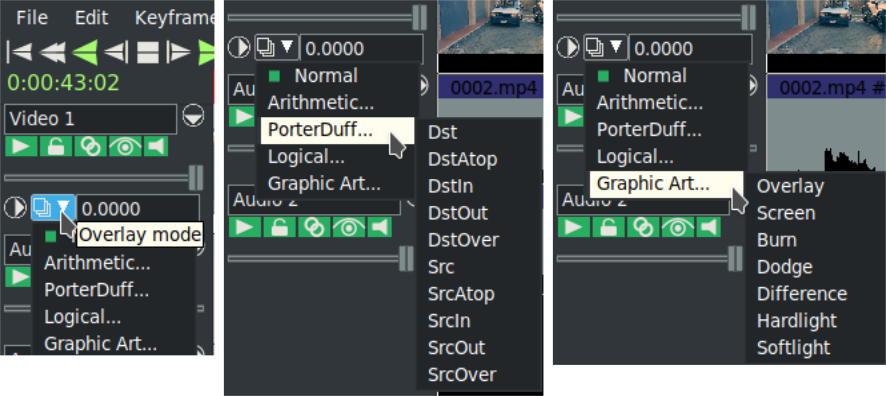
\includegraphics[width=0.99\linewidth]{images/overlay-01.png}
    \caption{Patchbay pulldown with Porter Duff and Graphic Art overlays expanded}
    \label{fig:overlay-01}
\end{figure}

Porter-Duff is the industry standard for alpha blending operations.  Only a short explanation follows here, but there is much more information to be found on the internet with complete descriptions and examples.  Every pixel has 3 color channels (like RGB), and may have 1 alpha channel value.  If there is no alpha defined for a color model, the alpha value is assumed to be 1.  Regions of the image are created with the alpha image map.  These regions are manipulated using the blending operations described below.  Alpha blending is the process of combining a foreground color with a background color which produces a new blended color.  The \textit{alpha} channel describes how much opacity is present in a pixel.  It may be completely transparent, completely opaque, or any range of translucency.

Conceptually, when the foreground color is completely opaque, the resulting blended color will be the foreground color.  If it is transparent, the blended color will be the color of the background.  When the value of the alpha channel is $1$, the image is all there, if it is $0$, there is no image at all, otherwise it is only partially there.  In other words, the alpha value goes from $0$ to $1$, where full transparency is $0$ and opaque is represented by $1$.  Alpha blending models opacity. 

When blending source and destination shapes (Dst and Src), the shape boundaries can be changed with the alpha blending effects.  There are a total of 10 standard Porter-Duff operators, but there are 30 possible overlay modes used in \CGG{}.  Each is characterized by its value in the four regions: source, destination and both, with the \textit{neither} region always being blank.  The source and destination regions can either be blank or filled with the source or destination colors.  A specific compositing math formula is used to calculate effect.  This is only applicable to RGB; some effort has been made to accommodate YUV, but the effects are not as predictable, and may not be useful. 

Below, in figure~\ref{fig:normal}, are the results of utilizing the 30 available operations within \CGG{} as listed on a following page.  Src is the solid green rectangle and Dst is the solid red rectangle.  There are better illustrations of what alpha blending can do, however for consistency sake, these are the results when using standards.

\begin{figure}[htpb]
    \centering
    \includegraphics[width=0.84\linewidth]{images/normal.png}
    \caption{Normal and Arithmetic overlays}
    \label{fig:normal}
\end{figure}

\begin{figure}[htpb]
    \centering
    \includegraphics[width=0.84\linewidth]{images/porter-duff.png}
    \caption{Porter Duff overlays}
\end{figure}

\begin{figure}[htpb]
    \centering
    \includegraphics[width=0.84\linewidth]{images/logical.png}
    \caption{Logical overlays}
\end{figure}

\begin{figure}[htpb]
    \centering
    \includegraphics[width=0.84\linewidth]{images/graphic-art.png}
    \caption{Graphic Art overlays}
\end{figure}

\section{Math algorithms}%
\label{sec:math_algorithms}

The implementation math forms are subsequently listed, where:

\vspace{2ex}
\begin{lstlisting}[language=bash, numbers=none]
Legend:
D = Destination
S = Source
a = alpha
c = chroma (color)
|| = OR (logical operator); 
? : = if (true/false) ... then (conditional ternary operator)
\end{lstlisting}

Each line describes a pair with the left one for alpha and the right one for chroma.

\subsection*{Normal}%
\label{sub:normal}

\begin{description}
    \item[NORMAL:] $[Sa + Da \times (1 - Sa), Sc \times Sa + Dc \times(1 - Sa)])$
\end{description}

\subsection*{Arithmetic:}%
\label{sub:arithmetic}

\begin{description}
    \item[ADDITION:] $[(Sa + Da), (Sc + Dc)]$
    \item[SUBTRACT:] $[(Sa - Da), (Sc - Dc)]$
    \item[MULTIPLY:] $[Sa + Da - Sa \times Da, Sc\times(1 - Da) + Dc\times (1 - Sa) + Sc \times Dc]$
    \item[DIVIDE:] $[Sa + Da - Sa \times Da, Sc\times(1 - Da) + Dc \times (1 - Sa) + Sc/Dc]$
    \item[REPLACE:] $[Sa, Sc]$ (fade = 1)
\end{description}

\subsection*{Porter-Duff}%
\label{sub:porter-duff}

\begin{description}
    \item[DST:] $[Da, Dc]$
    \item[DST\_ATOP:] $[Sa, Sc \times (1 - Da) + Dc \times Sa]$
    \item[DST\_IN:] $[Da \times Sa, Dc \times Sa]$
    \item[DST\_OUT:] $[Da \times (1 - Sa), Dc \times (1 - Sa)]$
    \item[DST\_OVER:] $[Sa + Da - Sa \times Da, Sc \times (1 - Da) + Dc]$
    \item[SRC:] $[Sa, Sc]$
    \item[SRC\_ATOP:] $[Da, Sc \times Da + Dc \times (1 - Sa)]$
    \item[SRC\_IN] $[Sa \times Da, Sc \times Da]$
    \item[SRC\_OUT:] $[Sa \times (1 - Da), Sc \times (1 - Da)]$
    \item[SRC\_OVER:] $[Sa + Da - Sa \times Da, Sc + (1 - Sa) \times Dc]$   
\end{description}

\subsection*{Logical}%
\label{sub:logical}

\begin{description}
    \item[MIN:] $[min(Sa, Da), MIN(Sc, Dc)]$
    \item[MAX:] $[max(Sa, Da), MAX(Sc, Dc)]$
    \item[LIGHTEN:] $[Sa + Da - Sa \times Da, Sc \times (1 - Da) + Dc \times (1 - Sa) + max(Sc \times Da, Dc \times Sa)]$
    \item[DARKEN:] $[Sa + Da - Sa \times Da, Sc \times (1 - Da) + Dc \times (1 - Sa) + min(Sc \times Da, Dc \times Sa)]$
    \item[AND:] $[Sa \times Da, Sc \times Dc]$
    \item[OR:] $[Sa + Da - Sa \times Da, Sc + Dc - Sc \times Dc]$
    \item[XOR:] $[Sa + Da - 2 \times Sa \times Da, Sc \times (1 - Da) + Dc \times (1 - Sa)]$
\end{description}

\subsection*{Graphical Art}%
\label{sub:graphical_art}

\begin{description}
    \item[OVERLAY:] $[Sa + Da - Sa \times Da, Sc \times (1 - Da) + Dc \times (1 - Sa) + 2 \times Dc < Da \quad ? \quad 2 \times Sc \times Dc : Sa \times Da - 	2 \times s (Da-Dc) \times (Sa-Sc) ]$
    \item[SCREEN:] $[Sa + Da - Sa \times Da, Sc + Dc - (Sc \times Dc)]$ (same as OR)
    \item[BURN:] $[Sa + Da - Sa \times Da, Sc \times (1 - Da) + Dc \times (1 - Sa) + Sc \leqslant 0 \parallel Sc \times Da + Dc \times Sa \leqslant Sa \times Da \quad ? \quad	0 : (Sc \times Da + Dc \times Sa - Sa \times Da) \times Sa/Sc]$
    \item[DODGE:] $[Sa + Da - Sa \times Da, Sc \times (1 - Da) + Dc \times (1 - Sa) + Sa \leqslant Sc \parallel Sc \times Da + Dc \times Sa \geqslant Sa \times Da \quad ? \quad	Sa \times Da : Dc \times Sa / (1 - Sc/Sa)]$
    \item[DIFFERENCE:]~\\ $[Sa + Da - Sa \times Da,  Sc \times (1 - Da) + Dc \times (1 - Sa) + abs{(Sc \times Da - Dc \times Sa)}]$
    \item[HARDLIGHT:] $[Sa + Da - Sa \times Da, Sc \times (1 - Da) + Dc \times (1 - Sa) + 2 \times Sc < Sa \quad ? \quad 2 \times Sc \times Dc : Sa \times Da - 	2 \times (Da - Dc) \times (Sa - Sc)]$
    \item[SOFTLIGHT:] $[Sa + Da - Sa \times Da, Sc \times (1 - Da) + Dc \times (1 - Sa) + Da > 0 \quad ? \quad (Dc \times Sa + 2 \times Sc \times (Da - 	Dc))/Da : 0]$
\end{description}

\section{Description}%
\label{sec:description}

The previous math forms are the only truly accurate description of each blending operation, but short descriptions are below where \textit{Source} is the output from the next track and \textit{Destination} is the output from the lower track stacking.  Blending starts with new Source and combines it with the previous render stack output, which is referred to as Destination.  The new output becomes the next Destination and the next up stack level becomes the new Source.  Source is above; Destination is below.

Note: the Graphic Art group operates principally on color, and the others operate principally on alpha.

\subsection*{Normal}%
\label{sub:normal2}

\begin{description}
    \item[Normal:] Normal mode is the default layer mode.  The result color is the source color.  The layer on top covers the layers below it.  If you want to see anything below the top layer when you use this mode, the layer must have some transparent areas.  It is \textit{stacked on top}.  Math formula used is different than that used by Gimp; there is no SVG equivalent.
\end{description}

\subsection*{Arithmetic Group:}%
\label{sub:arithmetic_group}

Standard numerical operations.

\begin{description}
    \item[Addition:] The source is added to the destination and replaces the destination.  Addition mode is very simple - the pixel values of the upper and lower layers are added to each other.  The resulting image is normally brighter.  The equation can result in color values greater than $255$, so some of the light colors may be clipped to the maximum value of $255$.  Math formula is the same as that used by SVG but different than Gimp.
    \item[Subtract:] Subtract mode reduces the pixel values of the upper layer by the pixel values of the lower layer.  The resulting image is normally darker.  You might get a lot of black or near-black in the resulting image.  The equation can result in negative color values, so some of the dark colors may be clipped to the minimum value of $0$.  Math formula used is different than that used by Gimp; there is no SVG equivalent.
    \item[Multiply:] The source color is multiplied by the destination color and replaces the destination.  The resulting color is always at least as dark as either the source or destination color.  Multiplying any color with black results in black.  Multiplying any color with white preserves the original color.  Math formula is the same as used by SVG and Gimp.
    \item[Divide:] Divides source color by destination color.  If the source color is white, the result color is the underlying color.  The resulting image is often lighter.  Math formula used is different than that used by Gimp; there is no SVG equivalent.
    \item[Replace:] Replace mode will cause any existing destination to be replaced by the source media.  Mathematical formula used is the same as used by Gimp; there is no SVG equivalent.
\end{description}

\subsection*{Porter-Duff Group}%
\label{sub:porter-duff_group}

Industry standard compositing operators.

\begin{description}
    \item[DST:] The destination is left untouched.  Only the destination will be present in the output.  Math formula is the same as that used by Porter-Duff and SVG; there is no Gimp equivalent.
    \item[DST\_ATOP:] The part of the destination lying inside of the source is composited over the source.  The destination outside the source is dropped.  You will see the existing canvas is only kept where the shapes overlap.  Math formula is the same as that used by Porter-Duff and SVG; there is no Gimp equivalent.
    \item[DST\_IN:] The part of the destination lying inside of the source is displayed.  This effectively allows for cutting out the background using the current layer/feature as a mask.  You will see the new shape is drawn only where both the source and the destination overlap.  Math formula is the same as that used by Porter-Duff and SVG; there is no Gimp equivalent.
    \item[DST\_OUT:] The part of the destination lying outside of the source is displayed.  This is basically a reverse mask, compared to destination-in.  You will see the existing content is kept where it doesn't overlap the source.  Math formula is the same as that used by Porter-Duff and SVG; there is no Gimp equivalent.
    \item[DST\_OVER:] The destination is composited over the source.  Math formula is the same as that used by Porter-Duff and SVG; there is no Gimp equivalent.
    \item[SRC:] The source is copied.  The destination is not used as input.  Only the source will be present in the output.  Math formula is the same as that used by Porter-Duff \& SVG; there is no Gimp equivalent.
    \item[SRC\_ATOP:] The part of the source lying inside of the destination is composited over the destination. The source outside the destination is dropped.  You will see the existing canvas is only kept where the shapes overlap.  Math formula is the same as that used by Porter-Duff and SVG; no Gimp equivalent.
    \item[SRC\_IN:] The part of the source lying inside of the destination is displayed.  This effectively allows the destination to act as a mask for the layer/feature being shown.  You will see the new shape is drawn only where both the source and the destination canvas overlap.  Math formula is the same as that used by Porter-Duff and SVG; there is no Gimp equivalent.
    \item[SRC\_OUT:] The part of the source lying outside of the destination is displayed.  This is basically a reverse mask, compared to source-in.  You will see the new shape is drawn where it doesn't overlap the destination.  Math formula is the same as that used by Porter-Duff and SVG; there is no Gimp equivalent.
    \item[SRC\_OVER:] The source is composited over the destination.  Math formula is the same as that used by Porter-Duff and SVG; there is no Gimp equivalent.
\end{description}

\subsection*{Logical Group}%
\label{sub:logical_group}

\begin{description}
    \item[Min:] The output color is the component-wise minimum value of the source and destination colors.  There is no SVG or Gimp equivalent math formula.
    \item[Max:] The output color is the component-wise maximum value of the source and destination colors. There is no SVG or Gimp equivalent math formula.
    \item[Lighten:] Selects the lighter of the destination and source colors.  The destination is replaced with the source when the source is lighter, otherwise it is left unchanged.  Completely black layers have no effect on the final image and completely white layers result in a white image.  Math formula is the same as used by SVG and Gimp's \textit{lighten only}.
    \item[Darken:] Selects the darker of the destination and source colors. The destination is replaced with the source when the source is darker, otherwise it is left unchanged.  Completely white layers have no effect on the final image and completely black layers result in a black image.  Math formula is the same as used by SVG and Gimp's \textit{darken only}.
    \item[And:] This operation intersects source and destination.  If either image is not white, it down factors the other image.  Usually you will end up with a lot of darker areas.  There is no SVG or Gimp equivalent math formula.
    \item[Or] This operation is the union of the source and the destination.  If either image is not black, it adds to the other image.  Usually you will end up with a lot of lighter areas.  Math formula is the same as that used by “Screen” operation in SVG; there is no Gimp equivalent.
    \item[Xor:] The union of the source and destination with the intersection removed.  Results in black if they are equal.  Shapes are made transparent where both overlap, and drawn normal everywhere else.  Math formula used is that used by Porter-Duff; there is no Gimp equivalent and SVG formula differs.
\end{description}

\subsection*{Graphical Art Group}%
\label{sub:graphical_art_group}

Typical operations from popular \textit{paint} packages.

\begin{description}
    \item[Overlay:] Multiplies or screens the colors, dependent on the destination color. Source color overlay the destination while preserving its highlights and shadows.  The destination color is not replaced, but is mixed with the source color to reflect the lightness or darkness of the destination.  Dark parts on the base layer become darker, and light parts become lighter.  Math formula is same as SVG and Gimp.
    \item[Screen:] The source and destination are complemented and then multiplied and then replace the destination.  The resultant color is always at least as light as either of the two constituent colors.  Screening any color with white produces white.  Screening any color with black does not change the other layer.  Using the Screen mode is similar to projecting multiple photographic slides simultaneously onto a single screen.  A lighter picture is the result.  Math formula is the same as used by SVG and Gimp.  This is identical to \textit{OR}.
    \item[Burn:] Darkens the destination color to reflect the source color.  Burning with white produces no change.  In photography, burning is a technique used in a darkroom to increase the exposure in particular areas of the image.  This brings out details in the highlights.  Math formula is the same as used by SVG and Gimp.
    \item[Dodge:] Brightens the destination color to reflect the source color.  Dodging with black produces no change.  The result color is a lightening of the source color to reflect the underlying layer color by decreasing the contrast.  If the source color is pure black, the result color is the underlying color.  In photography, dodging is a technique used in a darkroom to decrease the exposure in particular areas of the image.  This brings out details in the shadows.  Math formula is the same as used by SVG and Gimp.
    \item[Difference:] Subtracts the darker of the two constituent colors from the lighter.  This is the same as \textit{Subtract} except that the absolute value is used.  \textit{Subtract} colors which would be black due to clipping become visible instead.  Differencing with white inverts the destination color.  Differencing with black produces no change.  Math formula is the same as used by SVG and Gimp.
    \item[Hardlight:] Multiplies or screens the colors, dependent on the source color value.  If the source color is lighter than $0.5$, the destination is lightened as if it were screened.  If the source color is darker than $0.5$, the destination is darkened, as if it were multiplied.  The degree of lightening or darkening is proportional to the difference between the source color and $0.5$.  If it is equal to $0.5$ the destination is unchanged.  Using pure black or white produces black or white.  The effect is similar to shining a harsh spotlight on the destination.  This mode is useful for creating the appearance of shadows on a layer.  You might use this mode to combine two photographs and obtain bright colors and sharp edges.  Math formula is the same as used by SVG and Gimp.
    \item[Softlight:] Darkens or lightens the colors, dependent on the source color value.  If the source color is lighter than 0.5, the destination is lightened. If the source color is darker than $0.5$, the destination is darkened, as if it were burned in.  The degree of darkening or lightening is proportional to the difference between the source color and $0.5$.  If it is equal to $0.5$, the destination is unchanged.  Using pure black or white produces a distinctly darker or lighter area, but does not result in pure black or white.  The effect is similar to shining a diffused spotlight on the destination.  A layer with pure black or white becomes markedly darker or lighter, but does not become pure black or white.  Soft light is not related to “Hard light” in anything but the name, but it does tend to make the edges softer and the colors not so bright.   Math formula is the same as used by Gimp; SVG formula differs.
\end{description}

